\documentclass[a4paper, 12pt]{article}
\usepackage[utf8]{inputenc}
\usepackage{graphicx}
\usepackage[a4paper,left=1.25in,right=1in,top=1in,bottom=1in]{geometry}
\usepackage{tikz}
\usetikzlibrary{positioning,shapes,fit,arrows}
\usepackage{fancyhdr}
\usepackage{booktabs}
\usepackage{mathtools}
\usepackage{amsmath}
\usepackage{etoolbox}
\usepackage{caption}
\usepackage[ruled,vlined]{algorithm2e}
\usepackage{algorithm}
\usepackage{algorithmicx}
\usepackage{float}
\floatstyle{boxed} 
\restylefloat{figure}
\pagestyle{fancy}
\fancyhf{}
\fancyhead[LE,RO]{\footnotesize \center Botnet Detection using Machine Learning }
\fancyfoot[CE,CO]{\raggedright{P:F-SMR-UG/08/R0} }
\fancyfoot[LE,RO]{\thepage}

\begin{document}
 
\begin{titlepage}
    \begin{center}
        \vspace*{1cm}
        
        \large
        \textbf{Pune Institute of Computer Technology}	
        \linebreak
		\textbf{Dhankawadi, Pune}
        \vspace{0.5cm}
        \linebreak
        \linebreak
        \textbf{A SEMINAR REPORT }
        \linebreak
        \textbf{ON }
        \linebreak
        \vspace{0.5cm}
        \large
        \\Botnet Detection using Machine Learning
        \linebreak
        \linebreak
		
		\textbf{SUBMITTED BY}
		\vspace{1cm}
		
        \textbf{ Shreyas Nikam }
        \\ Roll No. 31241
        \\ TE-2
        \linebreak
        \linebreak
		        
        \textbf{\large{Under the guidance of}}
		\linebreak
	    Prof. Rekha A. Kulkarni
		\linebreak
        
        \vspace{0.8cm}
        
        
\includegraphics[scale=0.6]{pict}   
        
        \Large
        DEPARTMENT OF COMPUTER ENGINEERING\\
        
		\textbf{Academic Year 2019-20}
        
    \end{center}
\end{titlepage}
\pagebreak

\begin{titlepage}
\begin{center}
    
\includegraphics[scale=0.6]{pict} 
	\linebreak
	\Large
        DEPARTMENT OF COMPUTER ENGINEERING\\
        \textbf{Pune Institute of Computer Technology}
		\linebreak
		\textbf{Dhankawadi, Pune-43}
		\vspace{0.8cm}
		\Large
		
	    \textbf{CERTIFICATE}
	    		\linebreak
	    \linebreak
		This is to certify that the Seminar report entitled
        \linebreak
		\linebreak
		\large
		\textbf{“Botnet Detection using Machine Learning”}
		\linebreak
		\linebreak
		Submitted by
		\linebreak
		Shreyas Nikam \hspace{10mm}   Roll No. 31241 \linebreak
		\linebreak
		has satisfactorily completed a seminar report under the guidance of Prof. Rekha A. Kulkarni  towards the partial fulfillment of third year Computer Engineering Semester II, Academic Year 2019-20 of Savitribai Phule Pune University. 
		\linebreak
		\linebreak
		\linebreak
		\linebreak
		\linebreak
		\begin{table}[h]
		\begin{tabular}{ccc}
		Prof. Rekha A. Kulkarni    &                        &  \hspace{52mm} Prof. M.S.Takalikar\\
		Internal Guide      &                     &    \hspace{52mm} Head \\
		          &                         &       \hspace{47mm} Department of Computer Engineering \\
                    &                       & \hspace{52mm} 
		\end{tabular}
		\end{table}
		\end{center}
Place:\\
Date:

\end{titlepage} 

\pagenumbering{Roman}
\section*{ACKNOWLEDGEMENT}

\hspace{0.5cm} I sincerely thank our Seminar Coordinator Prof. B.D.Zope and Head of Department Prof. M.S.Takalikar
for their support.
\vspace{0.25cm}
\par I also sincerely convey my gratitude to my guide Prof. Rekha A. Kulkarni, Department of Computer Engineering for her constant
support, providing all the help, motivation and encouragement from beginning till end to make this seminar a grand success.
\vspace{0.25cm}

\newpage
\tableofcontents

\newpage
\listoftables
\listoffigures

\newpage

\section*{Abstract}

\hspace{0.5cm}In recent years, the botnets have been the most common threats to network security since it exploits multiple malicious codes like a Worms, Trojans, Rootkit, etc. The botnets have been used to carry phishing links, to perform attacks and provide malicious services on the internet. A lot of security approaches have been proposed in the area, but still, it is a challenging issue to detect modern botnets that are continuously improving for evading detection.
\par 
A social botnet refers to a group of social bots under the control of a single bot-master, which collaborate to conduct the same malicious activities. Using social botnets, spammers are now able to flood news and political websites with tens of thousands of comments. Since Twitter is a micro-blogging social media website, Twitter bots can be used to shift public opinion.
\par
In this seminar, I try to apply various machine learning techniques and algorithms to build a Twitter Bot Classifier.
\section*{Keywords}
Botnet, Machine Learning, Botnet Detection, Twitter Bots, Network Security, Cyber Security.
\newpage
\pagenumbering{arabic}


\begin{center}
\section{INTRODUCTION}
\end{center}
\subsection{Bots}
\par
\hspace{0.5cm}
A bot is nothing but a software application that is programmed and instructed to do a certain task. Bots are automated, and are made to do the same repetitive tasks and they run according to their instructions without human user interaction. Bots usually operate over the network like Chatbots, Webcrawlers, Social Bots, etc.
\par
Any automated actions by a bot that violate a website owner's intentions, the site's Terms of Service, or the site's Robots.txt rules for bot behavior can be considered malicious. Bots that attempt to carry out cybercrime, such as identity theft or account takeover, are also "bad" bots. While some of these activities are illegal, bots do not have to break any laws to be considered malicious. In addition, other malicious bot activities include performing DoS and DDoS attacks, Credential Stuffing, Inventory Hoarding, Spamming, Email Address Harvesting and Click Fraud.
\\
\subsection{Botnet}
\par 
\hspace{0.5cm}
A botnet refers to a group of computers which have been infected by malware and have come under the control of a malicious actor. The term botnet is a portmanteau from the words robot and network and each infected device is called a bot. Self-propagating botnets recruit additional bots through a variety of different channels. Pathways for infection include the exploitation of website vulnerabilities, Trojan horse malware, and cracking weak authentication to gain remote access. Once access has been obtained, all of these methods for infection result in the installation of malware on the target device, allowing remote control by the operator of the botnet. Once a device is infected, it may attempt to self-propagate the botnet malware by recruiting other hardware devices in the surrounding network.

\subsubsection{Botnet attack types}
\par 
Once the botnet’s owner is in control of your computer, they usually use your machine to carry out other nefarious tasks. Common tasks executed by botnets include:
\begin{itemize}
    \item  Using your machine’s power to assist in distributed denial-of-service (DDoS) attacks to shut down websites.
    \item Emailing spam out to millions of Internet users.
    \item Generating fake Internet traffic on a third-party website for financial gain.
    \item Replacing banner ads in your web browser specifically targeted at you.
    \item Pop-ups ads designed to get you to pay for the removal of the botnet through a phony anti-spyware package.
\end{itemize}
\\

\subsection{Twitter Bots}
\par
\hspace{0.5cm}
A Twitter bot is a type of bot software that controls a Twitter account via the Twitter API. The bot software may autonomously perform actions such as tweeting, re-tweeting, liking, following, unfollowing, or direct messaging other accounts. The automation of Twitter accounts is governed by a set of automation rules that outline proper and improper uses of automation. Proper usage includes broadcasting helpful information, automatically generating interesting or creative content, and automatically replying to users via direct message. Improper usage includes circumventing API rate limits, violating user privacy, spamming, and sockpuppeting. 

\subsubsection{Features}
\par
The following includes some criteria that may indicate a Twitter account being a bot:
\begin{itemize}
    \item Periodic and regular timing of tweets.
    \item Whether the tweet content contains known spam and
    \item The ratio of tweets from mobile versus desktop, as compared to an average human Twitter user.
\end{itemize}

\subsubsection{Examples of Twitter Bots}
\begin{itemize}
    \item \textbf{@CongressEdits} and \textbf{@parliamentedits} posts whenever someone makes edits to Wikipedia from the US Congress and UK Parliament IP addresses, respectively
    \item \textbf{@Zeitansage} tweeted the current time in 2009 and 2010 for about 330.000 times, every minute.
    \item \textbf{@everyword} has tweeted every word of the English language. It started in 2007 and tweeted every thirty minutes until 2014
\end{itemize}



\newpage
\begin{center}

\section{MOTIVATION}

\end{center}
\par
\hspace{0.5cm}
One of the most dangerous and damaging attacks for organizations, nowadays, is the infection of machines that allow the creation of botnets. The attacker can have full access to these machines allowing the engagement of multiple damaging activities. These kinds of attacks are hard to prevent because, once a machine is infected, the attacker might issue commands to the zombie machine right away, causing immediate damage. Current defense mechanisms use tools that inspect payload of packets to detect potential information carried inside packets, which are rendered useless if the packets are ciphered. Botnets have ways to minimize their network fingerprint, and use obfuscation and encryption which makes the task harder for the defender.
\par
\hspace{0.5cm}
Twitter botnets have been an area of interest for security experts and the average user of the platform for some time now. Whether it’s spreading spam, advertising cryptocurrency scams or potentially influencing the democratic process, bots have become a key research area. Everyday, new bots and botnets are created and they use clever tactics to evade detection. As the number of botnet attacks has been increasing, it is very difficult to find devices without any vulnerability. 





\newpage
\begin{center}

\section{LITERATURE SURVEY}

\end{center}

The following is a literature survey of various references:


\begin{table}[h!]
 \caption{Literature survey}
 \hspace{-2cm}
\begin{tabular}{|l|l|l|l|l|l|}
\hline
No. 
& Title
& Description
& Findings
& Limitations
& Dataset
\\ \hline
1.  & \begin{tabular}[c]{@{}l@{}}“Detection of \\ Botnet Activity \\ via Machine\\ Learning”\end{tabular}                & \begin{tabular}[c]{@{}l@{}}Describes a \\ simple taxonomy\\ for data ex- \\ filtration \\ techniques.\end{tabular}                                         & \begin{tabular}[c]{@{}l@{}}Proposed a \\ solution to \\ the problem of \\ detecting botnet \\ activity using \\ machine learning\\ approach.\end{tabular} & \begin{tabular}[c]{@{}l@{}}Lot of fals-\\ positives, more \\ fine-tuning \\ required.\end{tabular}               & \begin{tabular}[c]{@{}l@{}}Publicly \\ available \\ dataset found at \\ the University \\ of New \\ Brunswick\end{tabular} \\ \hline
2.  & \begin{tabular}[c]{@{}l@{}}“It's All in a \\ Name: Detecting\\ and Labeling \\ Bots by Their \\ Name”\end{tabular} & \begin{tabular}[c]{@{}l@{}}Uses random \\ string detection \\ applied to \\ users’ names \\ to filter Twitter \\ streams for \\ bot accounts.\end{tabular} & \begin{tabular}[c]{@{}l@{}}This technique \\ is able \\ to easily \\ filter accounts \\ that are likely \\ bot accounts.\end{tabular}                      & \begin{tabular}[c]{@{}l@{}}Restrictions on \\ data sharing, \\ and not all bots \\ are the same.\end{tabular}    & Own dataset
\\ \hline
3.  & \begin{tabular}[c]{@{}l@{}}“Botnet \\ Campaign \\ Detection on \\ Twitter”\end{tabular}                            & \begin{tabular}[c]{@{}l@{}}A novel approach \\ to detecting bots \\ on twitter in near \\ real-time.\end{tabular}                                         & \begin{tabular}[c]{@{}l@{}}Used K-means \\ clustering to \\ classify botnets\\ in real time.\end{tabular}                                                 & \begin{tabular}[c]{@{}l@{}}Optimization \\ and \\ refinement \\ required.\end{tabular}                           & \begin{tabular}[c]{@{}l@{}}Combination \\ of 13 datasets\end{tabular}
\\ \hline
4.  & \begin{tabular}[c]{@{}l@{}}“An empirical \\ comparison of \\ botnet detection \\ methods”\end{tabular}             & \begin{tabular}[c]{@{}l@{}}Compares the \\ output of three \\ different botnet \\ detection \\ methods.\end{tabular}                                      & \begin{tabular}[c]{@{}l@{}}Simplified \\ comparison of \\ BClus, \\ CAMNEP \\ and Bothunter \\ methods.\end{tabular}                                      & \begin{tabular}[c]{@{}l@{}}Need for a \\ comparison \\ methodology \\ and a proper \\ error metric.\end{tabular} & Own dataset
\\ \hline

\end{tabular}
\end{table}                     




\newpage
\begin{center}
\section{A SURVEY ON PAPERS}
\end{center}
\subsection{A hybrid machine learning approach to network
anomaly detection}
\hspace{1cm} In this paper, they defined the information exfiltration issue and talked about certain methods that permit assailants to take information. They talked about why a portion of the present safeguard systems are insufficient in light of the fact that there are different approaches to exfiltrate information. Likewise, associations in some cases disregard the secretive parts of information exfiltration and use instruments that can be obsolete, not managing this kind of issue. They portrayed a basic scientific classification for information exfiltration systems presented a study on the same. The overview was separated into four subsections: Exfiltration Techniques, Exfiltration Detection Mechanisms, Botnet Data Exfiltration, and Machine Learning. 
\par
\hspace{0.5cm}
They also  proposed an answer for the issue of distinguishing botnet action, utilizing an AI approach. They focused on the qualities and practices of botnets and concentrated on the highlights permitting them to prepare a classifier. The framework was made out of five principle modules: 
\begin{enumerate}
    \item Data Collector
    \item Feature Extractor
    \item Classifier
    \item Evaluator and
    \item Decider
\end{enumerate}
\hspace{0.5cm} Then again, the outcomes from the classifier were empowering when the framework was confronted with particular botnets (precision around 0.97), specifically, those that they previously had information of. At the point when all the botnets found in the dataset were tried, the discovery rate was lower than when utilizing the cross approval methodology, arriving at 0.73 precision. Considering the entire dataset, the Decider experienced very difficulty in flagging effectively the machines, despite the fact that that assignment is done more earnestly and unrealistically.
\subsection{Its All in a Name: Detecting and Labeling Bots by their name.}
\par
\hspace{1cm}  
This paper focused on identifying and classifying bot accounts on Twitter by using their screen names. They observed that most of the screen names that were generated randomly consisted of lower and upper alpha-numeric characters of length 15 and mostly belonged to bots and not real accounts. Then they constructed  training data consisting of 200,000 non-random Twitter screen names (randomly sampled from Twitter and manually verified as non-random) and 200,000 randomly generated 15 digit (which was standardized later) strings and developed a combination of heuristic filtering and traditional machine learning models to label the string as random or not random by using \textbf{character n-gram} and \textbf{Shannon entropy} which gave solid results.


\subsection{Botnet Campaign Detection on Twitter}
\hspace{1cm}  
The attributes used in this paper's approach are analyzed by performing a simple comparison to determine whether they are the same as that tweet's neighbors' attributes. What makes it stand apart is not the attributes used, or even the specific combination, but rather that this approach does not analyze the data, history, or network of an account. Instead, it compares most attributes against the nearest N tweets as they appear in chronological order. It has the advantage of only requiring the data of N tweets to make a determination, as the only data considered is that of the nearest N tweets on a chronological scale. As this approach is designed for detecting bot-nets and spam campaigns, it will not detect a lone bot acting on its own. This approach has massive advantages by requiring so little data that it is non-computationally difficult. This also allows this program to analyze tweets in real-time.
\par
\hspace{0.5cm}
The determination of whether a user is a bot or not is done by a scoring system. A certain select parameters are chosen and are scored using a scale. If the account meets a certain threshold of this score, then it is classified as a bot.


\subsection{An Empirical Comparison of Botnet Detection Methods}
\par
\hspace{1cm}
This paper primarily focuses on comparison of three botnet detection methods (BClus, CAMNEP and BotHunter) using a good dataset and a proper error metric. It focuses on comparison so that new methods can be assessed objectively and the techniques can be improved further. 
\par
\hspace{0.5cm}
\textbf{CAMNEP}  models the normal behaviour of the network and labels deviations from normal behaviour as anomalous. \textbf{BClus} method is a behavioral-based botnet detection approach that creates models of known botnet behaviour and uses them to detect similar traffic on the network. It clusters the traffic sent by each IP address and to recognize which clusters have similar behaviour to botnet traffic.The \textbf{BotHunter} is a rather complex method which the detects the infection and coordination dialog of botnets by matching a state-based infection sequence model. 


\newpage
\begin{center}
\section{PROBLEM DEFINITION AND SCOPE}
\end{center}

\subsection{Problem Definition}

\hspace{1cm}
Apply various Machine Learning Algorithms and techniques to build a Twitter Bot Classifier.

\subsection{Scope}

\hspace{1.5cm} 
Most of the existing Twitter Bot Classifiers focus on numerical-statistical data such as the total count of followers of the account, the number of friends, the number of favourites, the number of statuses posted, and boolean data like whether or not the account is verified, if it has a profile image, a default profile and if it has an extended profile.
\par
\hspace{0.5cm}
None of these methods take into account the name of the user account and the screen names that is displayed. This can account as a factor to some extent, as most of the bots tend to use random string names, special characters, or string sequences which are rarely used by actual users.
\par
\hspace{0.5cm}
In this seminar, I try to take into account this feature and add it as an attribute by deciding a probability of the account name being generated by a bot and using that to add to the model's overall evaluation.



\newpage
\begin{center}
\section{DIFFERENT MACHINE LEARNING ALGORITHMS}
\end{center}

\subsection{Logistic Regression}
Logistic Regression is a Machine Learning classification algorithm that is used to predict the probability of a categorical dependent variable. In logistic regression, the dependent variable is a binary variable that contains data coded as 1 (yes, success, etc.) or 0 (no, failure, etc.). In other words, the logistic regression model predicts $P(Y=1)$ as a function of X. Logistic Regression is used when the dependent variable (target) is categorical. It is given as:

\vspace{0.2cm}
\hfil $y = p + e;$ \\
\vspace{0.3cm}
\hfil $log(\frac{p}{1-p}) = a + b_1 x_1 + b_2 x_2 + ... + e;$ \\
\vspace{0.2cm}
\hfil where p is probability of outcome.
\\
\subsection{Support Vector Machine (SVM)}
\par
\hspace{1cm}
A Support Vector Machine (SVM) is a discriminative classifier formally defined by a separating hyperplane. In other words, given labeled training data (supervised learning), the algorithm outputs an optimal hyperplane which categorizes new examples. In two dimensional space this hyperplane is a line dividing a plane in two parts where in each class lay in either side.
\par
\hspace{0.5cm}It is mostly used in classification problems. In this algorithm, we plot each data item as a point in n-dimensional space (where n is number of features you have) with the value of each feature being the value of a particular coordinate. It has high prediction accuracy and performance rate but is limited to two classified classes only.
For linear kernel the equation for prediction for a new input using the dot product between the input $x$ and each support vector $x_i$ is calculated as follows:
\vspace{0.2cm}
\par
\hfil $f(x) = B(0) + sum(ai * (x, x_i))$
\vspace{0.2cm}
\par
The polynomial kernel can be written as: 
\par
\vspace{0.2cm}
\hfil $K(x,x_i) = 1 + sum(x * x_i)^d$
\vspace{0.2cm}
\par
and exponential as 
\par
\vspace{0.2cm}
\hfil $K(x,x_i) = exp^(-gamma * sum((x — x_i²))$
\\
\subsection{Decision Tree Classifiers}
\par
\hspace{1cm}
A decision tree is a tree where each node represents a feature(attribute), each link(branch) represents a decision(rule) and each leaf represents an outcome(categorical or continues value).
It repetitively divides the working area (plot) into sub part by identifying lines. Operations are carried with optimization. Efficiency reduces with increase in dataset.
The whole idea is to create a tree like this for the entire data and process a single outcome at every leaf(or minimize the error in every leaf).
\\

\subsection{Random Forest Classifier}
\par
\hspace{0.5cm}
Random forests are a combination of tree predictors such that each tree depends on the values of a random vector sampled independently and with the same distribution for all trees in the forest. A random forest is a classifier consisting of a collection of tree structured classifiers ${ h(x,Θk ), k=1, ...}$ where the ${Θk}$ are independent identically distributed random vectors and each tree casts a unit vote for the most popular class at input $x$.
Briefly, Random forest builds multiple decision trees and merges them together to get a more accurate and stable prediction.

\subsection{Naive Bayes Classifier}
\par
\hspace{0.5cm}
Naive Bayes algorithm can be defined as a supervised classification algorithm which is based on Bayes theorem with an assumption of independence among features. Bayes Theorem helps us to find the probability of a hypothesis given our prior knowledge. Bayes theorem is given as:
\par
\vspace{0.2cm}

\hfil $P(A|B) = \frac{P(B|A)*P(A)}{P(B)}$
\par
\vspace{0.2cm}
It describes the probability of an event, based on prior knowledge of conditions that might be related to the event.


\newpage
\begin{center}
\section{METHODOLOGY}

\end{center}
\subsection{Workflow}
\hfil
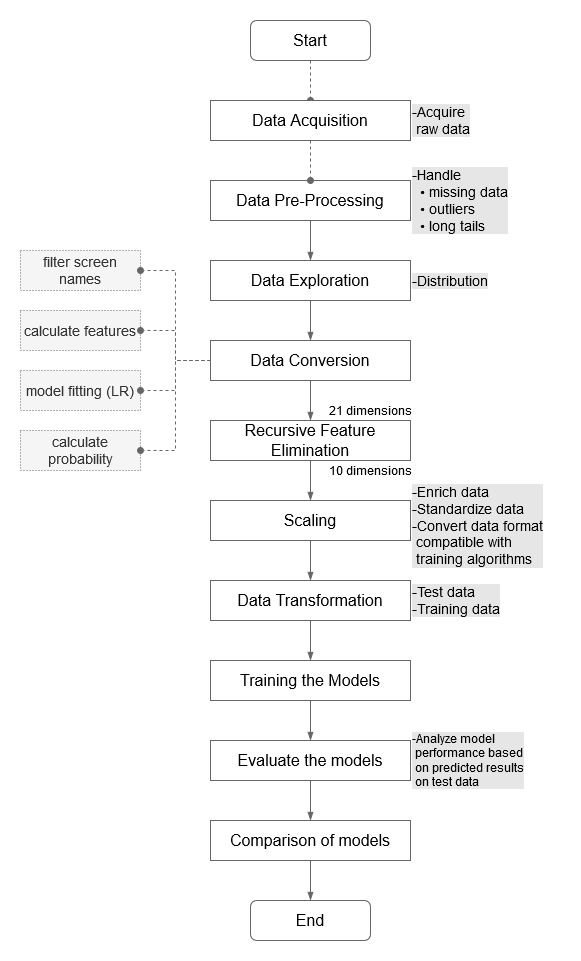
\includegraphics[scale = 0.6]{workflow}
\captionof{figure}{Workflow Diagram}


\begin{algorithm}[H]
\SetAlgoLined
dataset["namesProb"] = [ ]\; \\
temp = [ ]\; \\
\For{str in listofnames}{
    chars := 0\; \\
    digits := 0\; \\
    specialchars := 0\; \\
    hasbotsubstr = false\; \\
    \For{i in str}{ \\
        \If{i.isdigit()} {
            digits += 1 \;
            }
        \Else{
        \If{i.isalpha()}{
            chars += 1\; 
            }
        \Else{
        specialchars +=1\; \\
        }
        }
    }
    
    \If{str.lower().find("bot") != -1} {
        hasbotsubstr := true \; 
    }
    temp.append([chars,digits,specialchars,hasbotsubstr])
}
 scale temp between (0,1) \\
 logreg := LogisticRegressionCLassifier() \; \\
 logreg.fit(temp)\; \\
 prob := logreg.predict_probability()\; \\
 dataset["namesProb"] := prob \; \\
 \caption{Screen name conversion}
\end{algorithm}


\newpage
\section{Results}
\subsection{Comparison Table}
\hfil
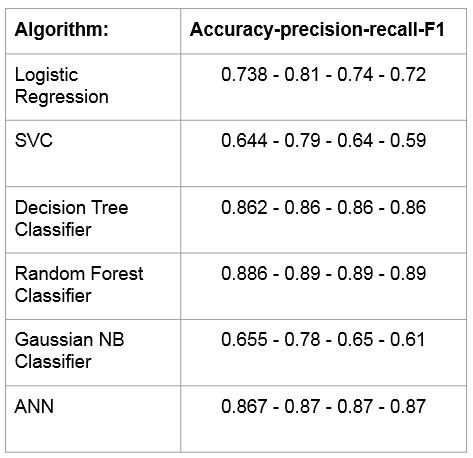
\includegraphics{comparison}
\captionof{figure}{Comparison of Accuracy, Precision, Recall and F1- Score of the various models that were implemented.}


\subsection{Implementation Results}
\hfil
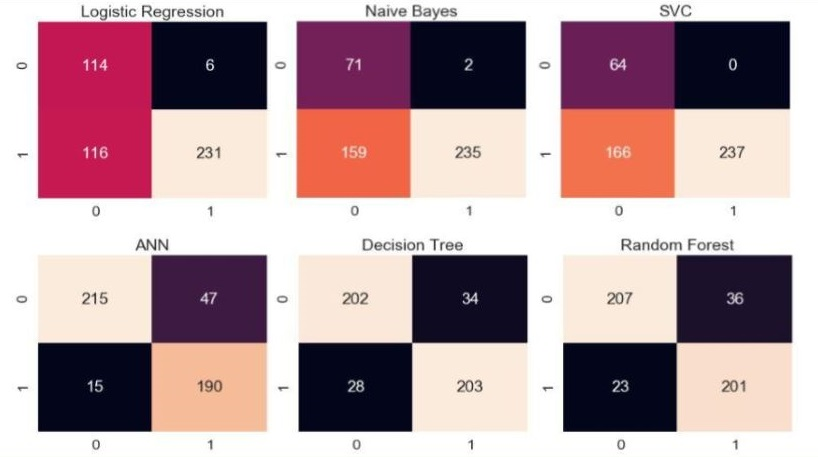
\includegraphics[scale=0.7]{confusion_matrices}
\captionof{figure}{Confusion matrices of each model.}
\vspace{1cm}
\hfil
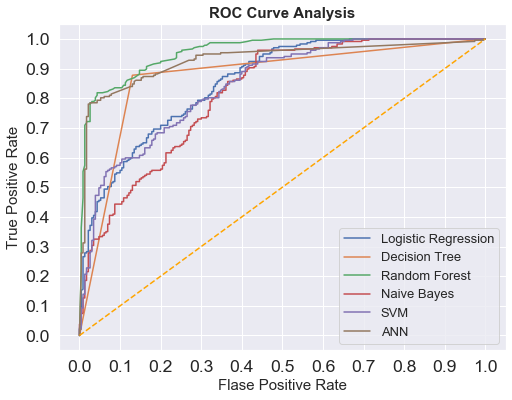
\includegraphics[scale = 0.8]{roc_curve}
\captionof{figure}{Receiver Operating Characteristic Curve of each model.}




\newpage
\begin{center}
\section{CONCLUSION}
\end{center}
\par
\hspace{1cm}
Using paper \cite{paper1} as base paper it was possible to implement various machine learning algorithms to classify between real Twitter accounts and bots. A comprehensive study of the comparison between the different models and their performance was also presented. Moreover, it was possible to extract features from the screen names using string detection as proposed in paper \cite{paper3} and further increase the accuracy of the model by 2-3\%.
\\
\begin{center}
\section{FUTURE SCOPE}
\end{center}
\par
\hspace{1cm}
This model was only implemented to detect bots from Twitter dataset. The model can be developed further for the detection of actual botnets on Twitter stream. Moreover, this can be done in real time by analyzing the behaviour of the account and these accounts which are termed as bots can be reported for suspension and/or deletion. All the attributes need to be further researched and refinements need to be done.
Fine tuning of parameters and optimization of code is needed.
\newpage

\addcontentsline{toc}{section}{References}
\bibliographystyle{plain}

\begin{thebibliography}{21}
\bibitem{paper1}  Jeremy D. Fields, “Botnet Campaign Detection on Twitter”, Department of Computer Science, SUNY Polytechnic, Marcy, NY, 2018.

\bibitem{paper2} Diogo Jeronimo, “Detection of Botnet Activity via Machine Learning”, Instituto Superior Tecnico, Lisboa, Portugal, November 2018.

\bibitem{paper3}  Beskow, David & Carley, Kathleen, “Its All in a Name: Detecting and Labeling Bots by Their Name”,  Computational and Mathematical Organization Theory. 25. 10.1007/s10588-018-09290-1.


\bibitem{paper4}  Hoang XD, Nguyen QC, “Botnet Detection Based On Machine Learning Techniques Using DNS Query Data”, Future Internet. 2018; 10(5):43.


\bibitem{paper5} S. Garcia, M. Grill, J. Stiborek, A. Zunino, “An empirical comparison of botnet detection methods”, Czech Technical University, Prague, May 2014


\bibitem{paper6} Chien-HauHung,Hung-MinSun , “A Botnet Detection System Based on Machine-Learning using Flow-Based Features”, National Tsing Hua University Hsinchu,Taiwan.


\bibitem{paper7}Shao-Chien Chen, Yi-Ruei Chen, and Wen-Guey Tzeng, “Effective Botnet Detection Through Neural Networks on Convolutional Features”, National Chiao-Tung University, Taiwan, IEEE, 2018

\bibitem{paper8}Manoj S. Koli, Manik K. Chavan, “An advanced method for detection of botnet traffic using Intrusion Detection System”, International Conference on Inventive Communication and Computational Technologies, ICICCT 2017.

\end{thebibliography}


\end{document}

